\documentclass[a4paper,titlepage,12pt]{article}
\usepackage[utf8x]{inputenc}
\usepackage[russian]{babel}
\usepackage{graphicx}
\usepackage{latexsym}
\usepackage{hyperref}
\usepackage{multirow}
\usepackage{multicol}
\usepackage{geometry}
\usepackage[version=3]{mhchem}
\usepackage{gensymb}

\graphicspath{{dot/}{gnuplot/}}

\geometry{top=3cm}
\geometry{bottom=3cm}
\geometry{left=3cm}
\geometry{right=2cm}

\title{Выделение и определение активности фруктозодифосфатальдолазы.\\
    Отчет за практикум по энзимологии}
\author{Студентов четвертого курса
    Мкртчяна Гарика и Нагаева Бориса}
\date{2011}

\begin{document}

\maketitle
\thispagestyle{empty}
\tableofcontents
\newpage


\section{Приготовление веществ}

Были приготовлены и убраны в холодильник следующие вещества:
\begin{enumerate}
\item Сульфат аммония, насыщенный раствор, pH 7.5
\item ЭДТА динатриевая соль, 5 mM раствор, pH 7.5
\item 5\% раствор аммиака (готовят из концентрированного аммиака, 25\%)
\item расвор сульфата аммония со степенью насыщения 0.52,
    приготовленный на 5\%-ном растворе аммиака
\item расвор сульфата аммония со степенью насыщения 0.5,
    приготовленный на 25 mM глицил-глициновом буфере, pH 7.5
\end{enumerate}

\subsection{Доведение pH концентрированных растворов}
\label{set-pH}
В некоторые растворы нельзя погружать электрод pH-метра,
так как эти растворы настолько концентрированны, что полученное значение pH будет неточным,
а электрод может быть попорчен.
Чтобы довести pH таких растворов до требуемого значения:
\begin{enumerate}
\item отобрать небольшую пробу, например, 2 ml
\item разбавить в 20 раз
\item погрузить электрод
\item довести pH до требуемого, прикапывая кислоту или щелочь
\item чтобы довести pH исходного раствора, следует добавить
     $ \frac{2}{3} \frac{V}{2\text{ml}} V_a$ кислоты или щелочи
     ($\frac{2}{3}$ -- эмпирическая величина), где:
     $ V $ -- объем исходного раствора,
     $ V_a $ -- объем добавленной кислоты или щелочи
\end{enumerate}


\section{Выделение фермента из скелетных мышц кролика (2 сентября)}
\subsection{Экстракция}
100 g мышц кролика было разрезано ножом и ножницами на фрагменты,
длина которых не превышала 5 мм.
В гомогенизатор с металлическими ножами было добавлено 150 ml ЭДТА, 5 mM, pH 7.5.
После этого фрагменты мышцы поместили в гомогенизатор и измельчали до тех пор,
пока вещество в гомогенизаторе не стало похоже на кашу.

Смесь была перемещена в стакан, после чего добавили ещё 75 ml охлежденного 5 mM ЭДТА, pH 7.5,
и перемешали в течение 10 минут.
Гомогенат пропустили через 4 слоя марли и процентрифугировали (20 минут при 18000 g).
Супернатант собрали. Объем супернатанта составил 240 ml.
Из супернатанта отобрали 500 мкл для анализов (\emph{проба 1}).

\subsection{Фракционирование}
\label{2-frac-end}
pH раствора был доведен до 7.5.
Для этого прикапывали равный объем (240 ml) холодного 5\%-ный аммиака
с помощью делительной воронки, при интенсивном перемешивании в течении 30(FIXME) минут.
Степень насыщения стала равной 0.5.
После этого оставили на 15 минут на холоде.

Затем раствор отцентрифугировали (20 минут при 18000g).
Супернатант собрали. Объем супернатанта составил 430 ml.
Из супернатанта отобрали 500 мкл для анализов (\emph{проба 2}).

Супернатант довели до степени насыщения 0.52 добавлением
насыщенного раствора сульфата аммония, pH 7.5 (4 ml  на каждые 100 ml раствора).
pH довели до 8.0 с помощью раствора сульфата аммония со степенью насыщения 0.52,
приготовленного на 5\%-ном растворе аммиака.
Данный раствор мог повредить электрод, поэтому придерживались
техники доведения pH концентрированных растворов (см. \ref{set-pH}).

Раствор оставили на сутки в холодильнике, ожидая появления кристаллов.


Однако кристаллы альдолазы так и не выпали.
Чтобы получить кристаллы, раствор довели до комнатной температуры,
после чего поставили в холодильник. Раствор помутнел.

Затем раствор центрифугировали (20 минут при 30000g).
Объем супернатанта составил 410 ml.
Из супернатанта отобрали 500 мкл для анализов (\emph{проба 3}).
Осадок перенесли в стеклянный стаканчик путем суспендирования осадка
в растворе сульфата аммония со степенью насыщения 0.5,
приготовленного на 25 mM глицил-глициновом буфере, рН=7.5.
Затем осадок, содержащий альдолазу, поместили в холодильник (\emph{проба 4}).
Объем осадка составил примерно 8 ml.

\section{Определение концентрации белка}

\subsection{Спектрофотометрическое опредление концентраций}
$$ A_{280} = \epsilon c l $$
Проверяли, что $ 0.1 < A_{280} < 1 $.

Для всех проб действовали по следующей схеме:
\begin{enumerate}
\item набирали 2 ml бидистилированной воды в кювету
\item обнуляли прибор
\item доливали 50 µl раствора из пробы
    (данное количество было подобрано, чтобы разведение составило 41).
\item снимали значение $A_{280}$
\end{enumerate}
Таким образом, разведение равно 41.
Было допущено, что удельное поглощение $\epsilon = 1$ для белка.
Для пробы 4 было использовано литературное значение $\epsilon = 0.91$.
Толщина кюветы $l = 1 \text{cm}$.
Таким образом, концентрация белка в пробе равна [mg/ml]:
$$ c=41 \cdot A $$

\begin{table}[htbp]
\caption{Концентрация белка, определенная спектрофотометрическим способом}
\begin{tabular}{|c|c|c|}
\hline
Проба & A & C[mg/ml] \\
\hline
1 & 0.49 & 20 \\
1 & 0.54 & 22 \\
\hline
2 & 0.177 & 7.257 \\
2 & 0.2 & 8.2 \\
\hline
3 & 0.154 & 6 \\
\hline
4 & 0.148 & 32.7 \\
\hline
\end{tabular}
\end{table}

\subsection{Введение в метод Брэдфорд}
Метод Брэдфорд -- один из колориметрических методов количественного определения белков в растворе
(особенно с низкой концентрацией).
Данный метод основан на связывании белками красителя Coomassie Brilliant Blue G-250 \cite{bradford-1}.
Механизм связывания Coomassie заключается во взаимодействии анионной формы красителя с белком \cite{bradford-2}.

\begin{figure}[htbp]
\def\svgwidth{0.7\linewidth}\input{img/Coomassie_Brilliant_Blue_G-250.pdf_tex}
\caption{Краситель Coomassie Brilliant Blue G-250}
\end{figure}

Связывание с белком осуществляется за счет электростатического взаимодействия сульфонильных групп
красителя с аминокислотными остатками белка.
Связывание красителя Coomassie происходит преимущественно с аргининовым остатком и в меньшей степени с
остатками гистидина, лизина, тирозина, триптофана и фенилаланина.
Количество связей, образуемых между Coomassie и белком, зависит от количества положительно заряженных групп,
расположенных в молекуле белка.
Считается, что 1.5-3 молекулы красителя связываются одной положительно заряженной группой \cite{bradford-3}.
Исходный кислый раствор Coomassie имеет максимум поглощения при длине волны 465 нм.
После связывания с белком и изменения окраски максимум поглощения смещается к 595 нм
(рисунок~\ref{fig-shift}).

\begin{figure}[htbp]
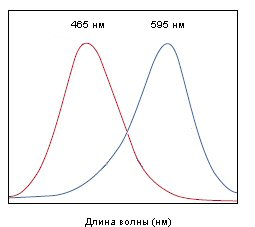
\includegraphics[width=0.4\linewidth]{bradford-shift}
\caption{Сдвиг максимума поглощения после связывания Coomasie с белком}
\label{fig-shift}
\end{figure}

\subsection{Калибровка для метода Брэдфорд}
\label{A0k}

Состав пробы: 1.9 ml Брэдфорд, буфер и БСА с концентрацией 0.4 mg/ml.

Под экспериментальные данные была подогнана линейная зависимость
(рисунок~\ref{fig-calibration}).

\begin{figure}[htbp]
\input{gnuplot/bsa}
\caption{Калибровка для метода Брэдфорд.
    На графике показана зависимость $A_{595}$ от содержания белка в кювете}
\label{fig-calibration}
\end{figure}

\subsection{Определение концентраций белка методом Брэдфорд}

Учитывая примерные концентрации, полученные спектрофотометрическим методом,
раствор из проб развели так, чтобы количество белка лежало в пределах
калибровочной кривой (0.1 -- 0.2).

Концентрация белка в пробе (mg/ml):

$$ c = \frac{m \cdot N}{V_c} $$
где $m$ -- содержание белка в кювете (µg),
$N$ -- разведение,
$V_c$ -- объем кюветы (2 ml).

\subsubsection{Проба 2}
Начали анализ с \emph{пробы 2}, в связи с чем потребовалось 4 попытки,
чтобы попасть в облась калибровочной кривой.

\def\svgwidth{\linewidth}\input{dot/br2-0.pdf_tex}

\def\svgwidth{\linewidth}\input{dot/br2-1.pdf_tex}
Содержание белка: $ m = \frac{A-A_0}{k} = 53.97 $ µg белка на кювету. \\
Разведение: $ N = 400 $ раз.
Концентарция белка в пробе: $ c = \frac{m \cdot N}{V_c} = 10.8 $ mg/ml.

\def\svgwidth{\linewidth}\input{dot/br2-2.pdf_tex}
Содержание белка: $ m = \frac{A-A_0}{k} = 35.32 $ µg белка на кювету. \\
Разведение: $ N = 1000 $ раз.
Концентарция белка в пробе: $ c = \frac{m \cdot N}{V_c} = 17.6 $ mg/ml.

\def\svgwidth{\linewidth}\input{dot/br2-3.pdf_tex}
Содержание белка: $ m = \frac{A-A_0}{k} = 25.07 $ µg белка на кювету. \\
Разведение: $ N = 2000 $ раз.
Концентарция белка в пробе: $ c = \frac{m \cdot N}{V_c} = 25.1 $ mg/ml.

Последние два опыта привели к желаемому результату
(A находится в области калибровочной прямой).

\subsubsection{Проба 1}
\def\svgwidth{\linewidth}\input{dot/br1.pdf_tex}
Содержание белка: $ m = \frac{A-A_0}{k} = 7.8 $ µg белка на кювету. \\
Разведение: $ N = 4000 $ раз.
Концентарция белка в пробе: $ c = \frac{m \cdot N}{V_c} = 15.6 $ mg/ml.

\subsubsection{Проба 3}
\def\svgwidth{\linewidth}\input{dot/br3.pdf_tex}
Содержание белка: $ m = \frac{A-A_0}{k} = 6.2 $ µg белка на кювету. \\
Разведение: $ N = 2000 $ раз.
Концентарция белка в пробе: $ c = \frac{m \cdot N}{V_c} = 6.2 $ mg/ml.



\end{document}

